\subsection{Recording}
The design choices for this concern is described in Section \ref{soc:recording}. To summarize, recording is the process of collecting and storing data received from sensors over an extended period. To enable a recording, we need to establish a connection with the available sensors and store the samples retrieved by the sensors on the device. In this thesis, we focus on collecting breathing data from the Flow sensor. Moreover, we will use the data streams dispatching module (hereafter: DSDM), which manages sensor discovery and sensor establishment to supported sensor sources, in our case the Flow sensor.  Moreover, the DSDM facilitates an interface for data acquisition, and the communication between the DSDM and Nidra occurs over IPC using binder's. During recording, we will check for connectivity with the sensors to ensure the sensors are collecting data at an appropriate rate. At the end of the recording, we will store metadata related to the recording and finalize the recording process. 

The functionality of recording can be separated into three actions: (A) start recording; (B) stop recording; and (C) display recording statistics. In the following sections, we will review the steps that enable these actions. 

\begin{figure}[!h]
    \centering
    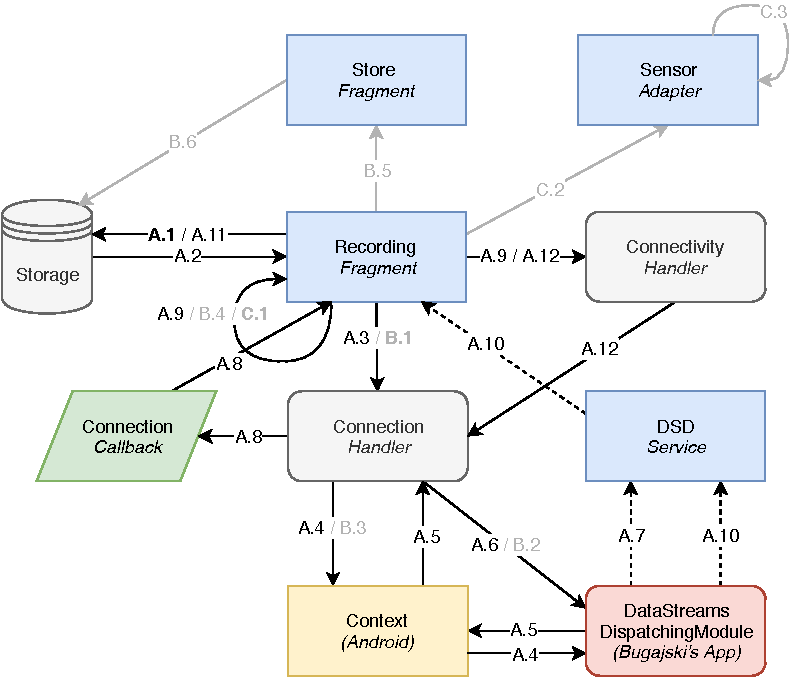
\includegraphics[scale=0.7]{images/Recording_ImpA.pdf}
    \caption{Implementation of recording functionality (A): start recording}
    \label{fig:impl_recordingA}
\end{figure}

\subsubsection{Action A: Start Recording}

In Figure \ref{fig:impl_recordingA}, an illustration of the component interactions are shown. Action A is to start a recording by connecting and starting data aqusition with the use of DSDM, and to ensure that the sensor source is gathering data at an appropriate rate. The steps and interactions for this action are: 

\begin{itemize}
    \item[A.1] The recording process starts by creating a new record entity that is inserted into the storage (see Section \ref{ioc:storage}). An empty record has to be inserted into the database in order to associate new samples with the record (based on the record's id). 
    \item[A.2] Once the record is inserted into the storage, a unique identification (id) is returned. 
    \item[A.3] \verb|ConnectionHandler| is invoked in order to manage the establishment, connection, and disconnection of the IPC between Nidra and DSDM service. The code for establishing the connection is described in the following listing (MainServiceConnection is the AIDL file as discussed in Section \ref{implement:aidl}):
\begin{lstlisting}[language=json, caption={}, captionpos=b]
    Intent intent = new Intent(MainServiceConnection.class.getName());
    intent.setAction("com.sensordroid.ADD_DRIVER");
    intent.setPackage("com.sensordroid");
    context.bindService(intent, serviceCon, Service.BIND_AUTO_CREATE);
\end{lstlisting}
    
    \item[A.4] If the service is offline when binding, the flag \verb|Service.BIND_AUTO_CREATE| will ensure for starting the service. \verb|BindService| allows components to send requests, receive responses, and perform inter-process communication (IPC) based on the interface provided by the host service (DSDM). 
    \item[A.5] Once the service is bound, we can proceed to communicate with the DSDM service. 
       \item[A.6] The \verb|ConnectionHandler| proceeds to initialize the connection with the sensor through the DSDM.  A request to the DSDM for available publishers with \verb|getPublishers()| is made, to retrieve all available sensor publishers connected to the DSDM. Occasionally, the DSDM uses extended time to discover all of the active sensors connected to the device; therefore, we have an interval that checks whether DSDM has any available sensors connected. 
    \item[A.7] Moving on,  a request to the DSDM to \verb|Subscribe| to a sensor is made. We specify that we want the Flow sensor in the \verb|Subscribe| method, in addition, a reference to the package name (Nidra) and a service object (\verb|DSDService|). The service object is where all of the data packets from the subscribed Flow sensor is received (on the \verb|putJson()| method).   
    \item[A.8] Also, a callback to \verb|RecordingFragment| with information of the sensor source (i.e., Flow) that we subscribe to is made, in order to display the information on the user's screen. 
    \item[A.9] The recording has now started, and a timer to measure the time spent on the recording is started. The \verb|ConnectivityHandler| is also initialized, which actively checks that the samples arrive within a specified time frame (as discussed in the design, a frame of 10 seconds that increases throughout the recording). The \verb|ConnectivityHandler| is implemented with a \verb|Handler| with a \verb|PostDelay| that counts down to zero. Upon a sample arrival, the timer is reset. 
    \item[A.10] Periodically, the DSDM receives samples from the Flow sensor. DSDM forwards the sample from the sensor to the service object (\verb|DSDService|) on the \verb|putJson()| method. The DSDService uses a \verb|LocalBroadcastManger| to send the data packet to the \verb|RecordingFragment|. This process goes on infinitely unless the recording or the sensor has been stopped. 
    \item[A.11] \verb|RecordingFragment| listens for the events on the local broadcast receiver. Upon an event, the data that is received from the sensor is processed. In other words, we extract the samples from the data packet, and insert it as a new a new sample entity with the current record's id as an association. 
    \item[A.12] Recalling the functionality from step A.9; if the event for the \verb|PostDelay| is triggered, it is equivalent to a sample not being acquired from the sensor. Therefore, we try to reconnect with the subscribed sensor by disconnecting with the DSDM (which will close the connection with the sensor source), followed up by a reconnection with the DSDM and subscribing to the same sensor source. Most of the times, the process of reconnecting with the sensor one time solves the issue; however, some times the sensor might require to be reconnected with several times in order to work. 
\end{itemize}

\subsubsection{Action B: Stop Recording}
\begin{figure}
    \centering
    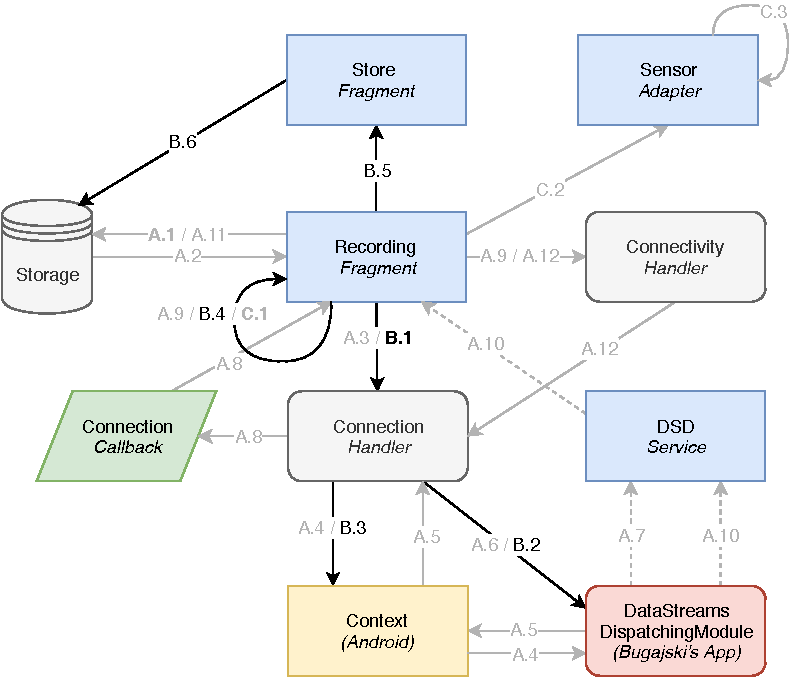
\includegraphics[scale=0.7]{images/Recording_ImpB.pdf}
    \caption{Implementation of recording functionality (B): stop recording}
    \label{fig:impl_recordingB}
\end{figure}

In Figure \ref{fig:impl_recordingB}, an illustration of the component interactions are shown. Action B is based on user input to stop the recording process. To the user, the recording has terminated, and the user is presented with a screen to provide extra information regarding the recording (e.g., title, description, and rating). For the application, it has to unsubscribe from the connected sensor sources (i.e., Flow), and disconnect the connectivity with the DSDM. Also, transition the user to the screen where the user can provide extra information that will be stored alongside the record.

\begin{itemize}
    \item[B.1] The user decides when to stop a recording with a press of a button. The event to stop the recording is sent to the \verb|ConnectionHandler|.
    \item[B.2] A call to the \verb|Unsubscribe()| method that contains the service object (i.e., DSDService) and the identification of the sensor source (e.g., Flow) is sent to DSDM. The DSDM has to ensure unsubscribing the sensor from a specific application and disconnect the IPC between the application. If there are no subscribing applications to the specific sensor source, the DSDM will signal the sensor to stop sampling and disconnect with the sensor. 
    \item[B.3] The IPC connection between Nidra and DSDM is discontinued by unbinding the service. 
    \item[B.4] The estimated time of recording is calculated, and a transition from \verb|RecordingFragment| to \verb|StoreFragment| is made to finalize the recording with extra information (e.g., title, description, and rating). 
    \item[B.5] The \verb|StoreFragment| uses the record identification retrieved on recording (A.1) in order to update the record with statistics and user-defined metadata. The statistics are the monitoring time, number of samples during recording, and retrieving the current state user biometrical data. The user-defined metadata are the title of the recording, a description enabling the user to add a note to the recording, and a rating between 1--5 (to give a rating on how the recording felt). 
    \item[B.6] The modified record is updated in the database, and the user is transitioned to the \verb|MainActivity|.
\end{itemize}

\begin{figure}[!h]
    \centering
    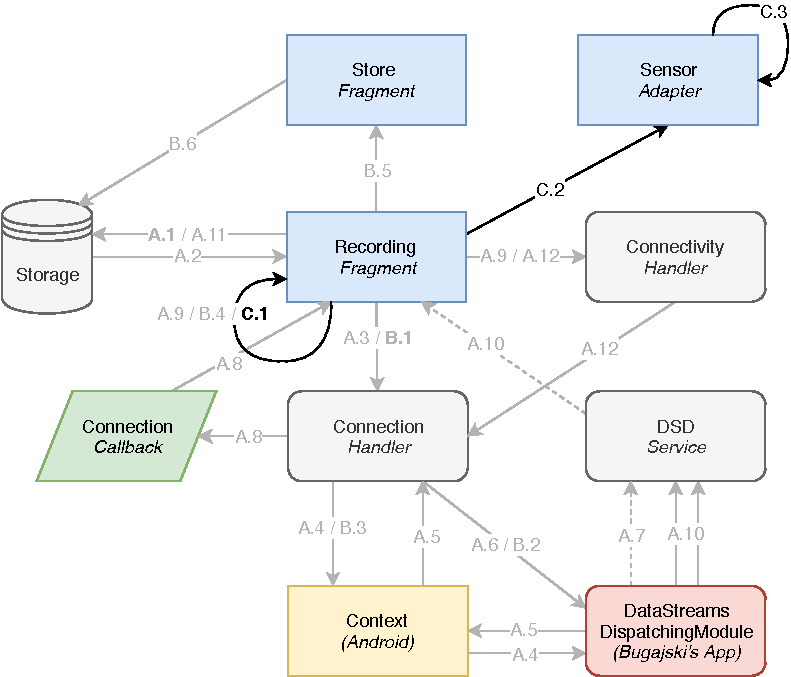
\includegraphics[scale=0.7]{images/Recording_ImpC.pdf}
    \caption{Implementation of recording functionality (C): display recording statistics}
    \label{fig:impl_recordingC}
\end{figure}


\subsubsection{Action C: Display Recording Statistics}
During a recording, the user can view the statistics for the recording. More specifically, the user can see the available connected sensors and a graph of the breathing data in real-time. In Figure \ref{fig:impl_recordingC}, an illustration of the component interactions are shown, and the steps and interaction for this action are: 


\begin{itemize}
    \item[C.1] The data is graphically represented as an intractable time-series graph. By using the GraphView library \cite{androidgraph}, we can in similarities to the implementation of the analytics concern (see Section \ref{ioc:analytics}), implement a graph to illustrate the breathing data to the user in real-time. As such, the user is presented with an interactable graph that continously updates with the samples acquired from the sensor.
    \item[C.2] In addition to the time-series graph, we have a list of publishers (e.g., Flow) that we acquired in the begging of the recording. As such, a list of publishers is sent to \verb|SensorAdapter|. 
    \item[C.3] The \verb|SensorAdapter| populates a view with the connected sensor to the user, in our case the Flow sensor. 
\end{itemize}


\subsection{Sharing}

The design choices for this concern is described in Section \ref{sec:design_sharing}. To summarize, sharing enables users to transmit records across application over a media (e.g., e-mail). The functionality of sharing is separated into two concerns, namely exporting and importing. The exporting consists of packing the records the user has selected for transmittal to another mobile device, while importing consists of locating the file on the user's device and parsing the data and storing in the database.

Before a user can proceed with these actions, the records from the database have to be presented. The \verb|FeedFragment| contains a \verb|RecyclerView| which populates the records into inside the \verb|FeedAdapter| (steps: 1-4). The adapter contains all the interactions and the event handling (e.g., button event listener for exporting) for a single record. 

The functionality of sharing can be separated into two actions: (A) exporting one or all records; and (B) import a record from the device. In the following sections, we will review the steps that enable these actions:


\begin{figure}
    \centering
    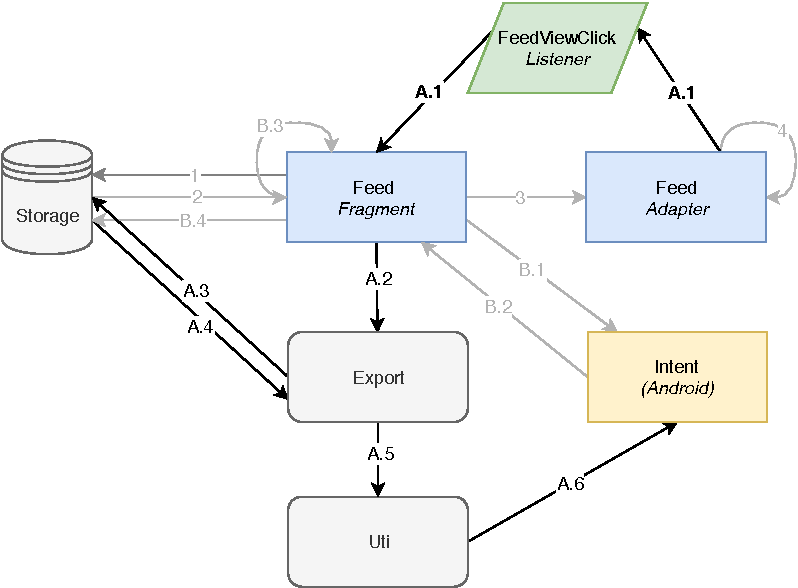
\includegraphics[scale=0.7]{images/Sharing_ImpA.pdf}
    \caption{Implementation of sharing functionality (A): exporting one or all records}
    \label{fig:impl_sharingA}
\end{figure}

\subsubsection{Action A: Exporting one or all Records}
In Figure \ref{fig:impl_sharingA}, an illustration of the steps to export one single recording is shown. However, the \verb|Feed Fragment| has an option to export all record; therefore, by disregarding the first step (A.1), the same structure applies to export all records. In essence, exporting consists of bundling the records and corresponding samples into a formatted file, and prompting the user with options to select a media (e.g., mail) for transmission. The steps can be narrowed down to: 

\begin{itemize}
    \item[A.1] Upon an event for exporting a selected record in \verb|FeedAdapter|, the record information is sent to the \verb|FeedFragment| through the callback reference (\verb|onRecordAnalyticsClick|) between these components. The record information will be used to determine the corresponding samples for the record.
    \item[A.2] The \verb|FeedFragment| sends the record information to the \verb|export| method inside of the \verb|Export| object, which is responsible for enabling the export. 
    \item[A.3] An operation to retrieve all samples related to the record (see: Section \ref{ioc:storage}) is done. 
    \item[A.4] The \verb|export| method retrieves all of the samples related to the record. Next, the record and the samples are encoded into an exportable JSON format (see: Section \ref{design:datapackets}). In order to share files between applications, the content has to be stored on the device. Thus, the encoded data is written into a file on the device, with a filename of \verb|record_(current_date).json|, and the next step uses the reference to the file location. 
    \item[A.5] The encoded file URI is retrieved with the use of \verb|FileProvider| (facilitates secure sharing of files across applications). The code snippet for this step is shown in the following listing: 
\begin{lstlisting}[language=json, caption={}, captionpos=b]
static void shareFileIntent(Activity a, File file) {
    Uri fileUri = FileProvider.getUriForFile(a.getApplicationContext(), a.getApplicationContext().getPackageName() + ".provider", file);

    Intent iShareFile = new Intent(Intent.ACTION_SEND);
    iShareFile.setType("text/*");
    iShareFile.putExtra(
        Intent.EXTRA_SUBJECT, "Share Records");
    iShareFile.putExtra(Intent.EXTRA_STREAM, fileUri);
    ...
    a.startActivity(
        Intent.createChooser(iShareFile, "Share Via"));
}

\end{lstlisting}

    \item[A.6] The user is displayed with a popup interface with several options to share the file over a media (e.g., e-mail). An illustration of the layout can be found in Section \ref{ioc:presentation}. 


\end{itemize}


\begin{figure}
    \centering
    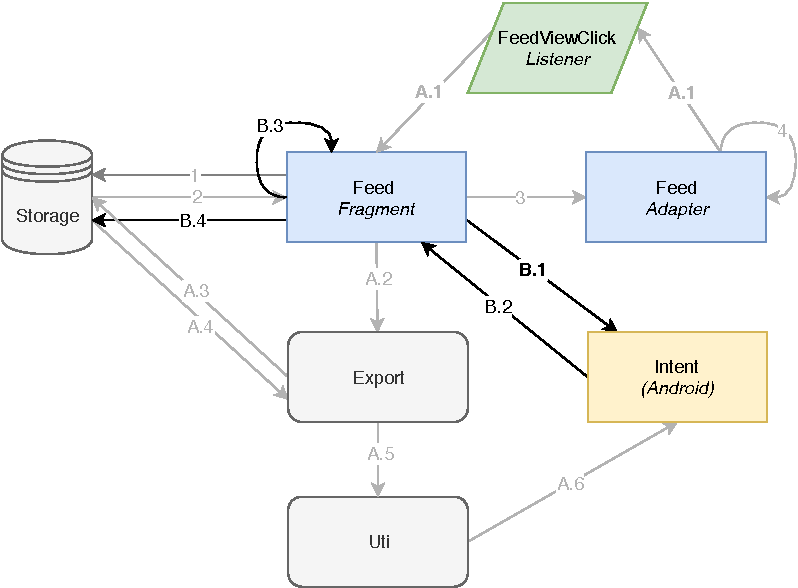
\includegraphics[scale=0.7]{images/Sharing_ImpB.pdf}
    \caption{Implementation of sharing functionality (B): import a record from the device}
    \label{fig:impl_sharingB}
\end{figure}

\subsubsection{Action B: Import a Record from the Device}
In Figure \ref{fig:impl_sharingB}, an illustration of importing a record from the device is shown. Importing consists of locating the formated file (the user has to obtain the file and store it on the device on beforehand), parsing the content in the file, and storing the data respective to the user's database. The steps can be narrowed down to:

\begin{itemize}
    \item[B.1] The user requests to view the import interface. The interface is provided by Android and allows the user to select files on the device. The code snippet for this step is shown in the following listing:
\begin{lstlisting}[language=json, caption={}, captionpos=b]
private void importRecords() {
    Intent intent = new Intent(Intent.ACTION_GET_CONTENT);
    intent.setType("*/*");
    startActivityForResult(intent, 1);
}

\end{lstlisting}
    \item[B.2] Once the user has selected the desired file, the method \verb|onActivityResult| inside of \verb|FeedFragment| is called, and location of the selected file can be obtained. 
    \item[B.3] The file location is an obscured path to the file on the device; thus, parsing the path with the use of \verb|Cursor| method (Android library) has to be done. After the absolute path is found, the data is decoded accordingly to the data format.
    \item[B.4] The record information and the samples are extracted from the decoded data. The information is then put into a new record entity alongside new samples entities, and are inserted into the user's database. 
\end{itemize}

\subsection{Modules}
The design choices for this concern is described in Section \ref{soc:modules}. To summarize, modules are standalone application that provides data enrichment or extended functionality to Nidra. For example, a module can use the records with samples provided by Nidra in order to feed a machine learning algorithm that predicts sleep apnea. Moreover, to add and launch a module from Nidra we need the modules package name. The package name and the name of the module-application is easily obtained within Android. 

The functionality of modules can be separated into two actions: (A) add a module; and (B) launch a module.  In the following sections, we will take a look into the steps that are taken to enable the actions.

\subsubsection{Action A: Add a Module}
In order to add a new module, the user has to install the module-application on the device beforehand. By listing through the installed application on the device, the user can select the desired module to be added in Nidra. In Figure \ref{fig:impl_modulesA}, an illustration of adding a module is shown, and the steps can be narrowed down to:

\begin{figure}
    \centering
    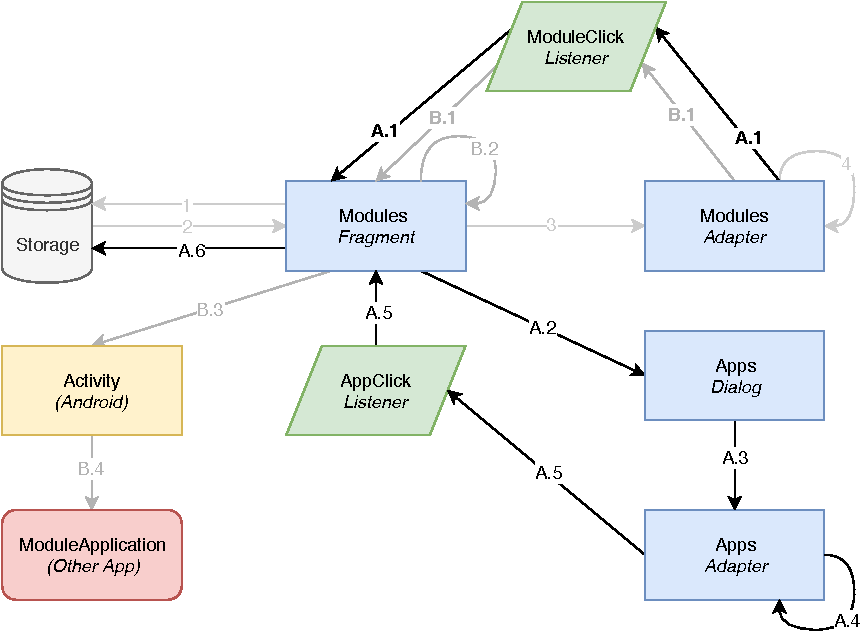
\includegraphics[scale=0.7]{images/Module_ImpA.pdf}
    \caption{Implementation of module functionality (A): add a module}
    \label{fig:impl_modulesA}
\end{figure}

\begin{itemize}
    \item[A.1] Upon an event for adding a new module in \verb|ModulesAdapter|, the \verb|ModulesFragment| is notified through the callback reference (\verb|onNewModuleClick()|) between these components.
    \item[A.2] The \verb|ModulesFragment| launches a custom Android dialog, which will list all of the installed application on the device. 
    \item[A.3] The \verb|AppsAdapter| will fetch all of the application that is not a system package, already an installed module, or the current application (Nidra). Next, the adapter for the dialog will be populated with the eligible applications. 
    \item[A.4] Once the user has selected the desired module-application, an event to the \verb|ModulesFragment| through the callback reference \verb|onAppItemClick()| between these components are made. The callback contains an Android object of \verb|PackageInfo| (contains the name and package name of the application) for the selected module-application.
    \item[A.5] The dialog is dismissed, and the application name and package name are extracted from the \verb|PackageInfo| for the selected module-application. 
    \item[A.6] Furthermore, the acquired information (i.e., name and package name) is stored in our database as a module entity. 
\end{itemize}

\begin{figure}[!h]
    \centering
    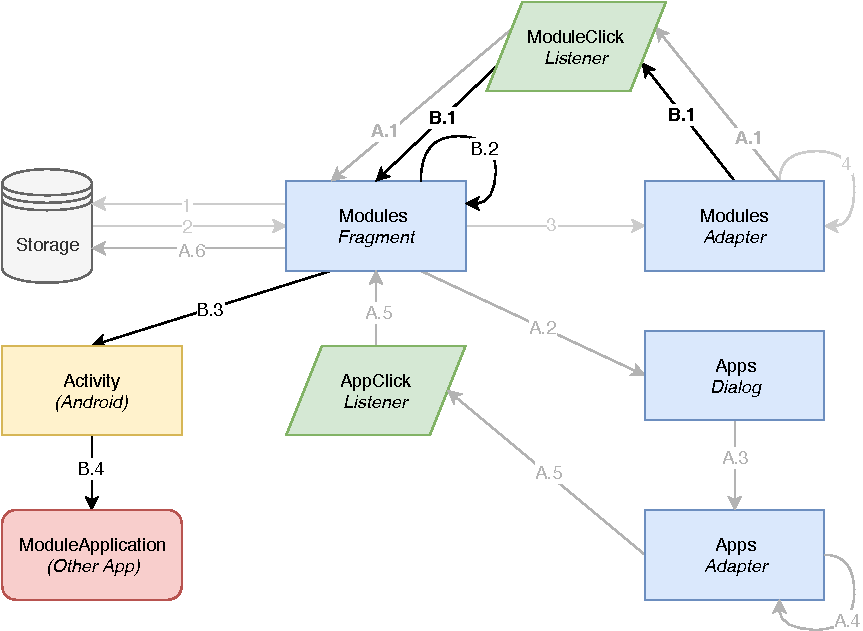
\includegraphics[scale=0.7]{images/Module_ImpB.pdf}
    \caption{Implementation of module functionality (B): launch a module}
    \label{fig:impl_modulesB}
\end{figure}

\subsubsection{Action B: Launch a Module}
A module is launched a separate application with a separate process, due to Android prohibits launching for other applications inside of an application. All added modules are listed and presented to the user on a separate screen. On the launch of a module, all records (including corresponding samples) in Nidra are encoded into a JSON format and bundled with the launch of the module. In Figure \ref{fig:impl_modulesB}, an illustration of launching a module, and the steps can be narrowed down to:

\begin{itemize}
    \item[B.1] Upon an event for launching a module in \verb|ModuleAdapter|, the package name of the module is sent to the \verb|ModulesFragment| through the callback reference (onLaunchModuleClick()) between these components. The package name will be used to launch the module-application.
    \item[B.2] All records (including their samples) on the device for the user, are formated into a JSON string and bundled into the launch. The code snippet for this step is shown in the following listing:
\begin{lstlisting}[language=json, caption={}, captionpos=b]
public void onLaunchModuleClick(String packageName) {
    Intent moduleApplication = context.getPackageManager().getLaunchIntentForPackage(packageName);

    if (moduleApplication == null) return;

    String data = formatAllRecordsToJSON();

    Bundle bundle = new Bundle();
    bundle.putString("data", data);

    moduleApplication.putExtras(bundle);

    startActivity(moduleApplication);
}
\end{lstlisting}

    \item[B.3] The activity uses the data provided in the \verb|Intent|, which includes the package name (the name of the module-application to determine the correct application) to launch the application with \verb|startActivity()|.
    \item[B.4] The selected module is then launched and presented to the user. The user can at anytime press the back button to return to Nidra.  
\end{itemize}

\begin{figure}
    \centering
    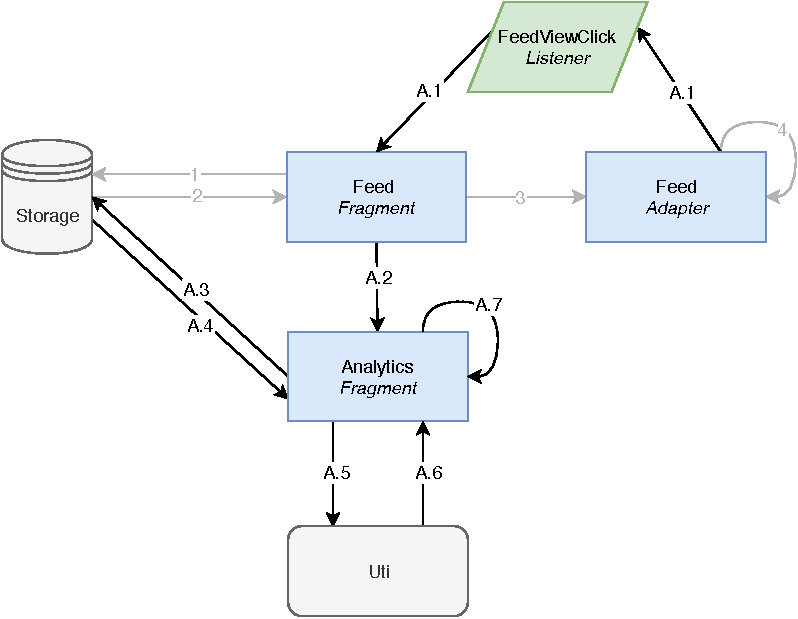
\includegraphics[scale=0.7]{images/Anal_Imp.pdf}
    \caption{Implementation of analytics functionality (A): display a graph for a single record}
    \label{fig:impl_analytics}
\end{figure}

\subsection{Analytics}\label{ioc:analytics}
The design choices for this concern is described in Section \ref{soc:analytics}. To summarize, analytics is the part of illustrating and analyzing the records. In Nidra, the analytics part of the implementation is limited to a time-series graph for a single record. While there are possibilities of extending the \verb|AnalyticsFragment| with other graphs based on the current structure, the facilitation of modules allows for easier integration of various analytical techniques and methods.

Similar to sharing, the records from the database have to be presented. The \verb|FeedFragment| contains a \verb|RecyclerView| which populates the records into inside the \verb|FeedAdapter| (steps: 1-4). The adapter contains all the interactions and the event handling (i.e., button event listener for analytics) for a single record. 

The functionality of analytics can be identified by one action: (A) display a graph for a single record to the user. In the following section, we will take a look into the steps that are taken to enable the action.

\subsubsection{Action A: Display a Graph for a Single Record}
Nidra provides a simple time-series graph of breathing data obtained during the recording. The graph data is plotted into a GraphView library \cite{androidgraph}, which enables interactions (e.g., zoom and scrolling) on the data samples. The X-axis is the breathing value based on the Y-axis of time of sampling. In Figure \ref{fig:impl_analytics}, an illustration of displaying a graph shown, and the steps can be narrowed down to:

\begin{itemize}
    \item[A.1] Upon an event for analytics on a selected record in \verb|FeedAdapter|, the record information is sent to the \verb|FeedFragment| through the callback reference (\verb|onRecordAnalyticsClick()|) between these components. The record information will be used to determine the corresponding samples for the record.
    \item[A.2] A new instance of the \verb|AnalyticsFragment| is created, and a transition from the \verb|FeedFragment| to the \verb|AnalyticsFragment| is made. Alongside, the record information is transmitted as a bundle.
    \item[A.3] An operation to retrieve all samples related to the record with the use of the \verb|SampleViewModel| is done. 
    \item[A.4] The \verb|AnalyticsFragment| retrieves all of the samples related to the record. The samples have to be structured according to the graph library to display an interactive time-series graph.
    \item[A.5] Each sample has to be extracted from the sample-data according to the sensor data structure (see Section \ref{design:datapackets}).
    \item[A.6] The sample value is returned and inserted into an array over data points used in the graph. 
    \item[A.7] The user is presented with a graph which is intractable. The Y-axis has the sample value on the given time (in HH:MM:SS) on the X-axis. The graph library enables interactions (e.g., zooming and scrolling) to gain a better understanding of the recording. 
\end{itemize}

\begin{figure}[!h]
    \centering
    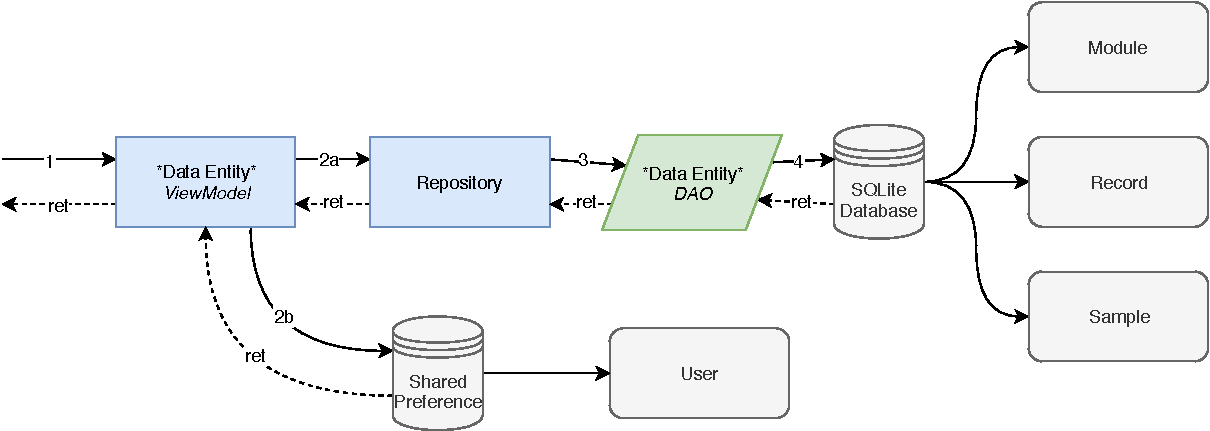
\includegraphics[scale=0.60]{images/Storage_Imp.pdf}
    \caption{Implementation of storage functionality}
    \label{fig:impl_storage}
\end{figure}

\subsection{Storage}\label{ioc:storage}

Storage facilities persistent data which remain on the device after application termination. In Nidra, there are four individual data entities (i.e., record, sample, module, and user). In Section \ref{soc:storage}, we discussed the design choices of storage possibilities for the individual data entity. To summarize, the entities of record, sample, and module are stored in a SQLite database, while the user entity is stored in a SharedPreference on the device.

The data entities has support for the standard CRUD operations (i.e., create, read, update, and delete); however, some of the entities has extra operations: record entity has an operation to retrieve all of the records on the user's device, sample entity has an operation to retrieve all of the samples for a given record (based on record's id); the module entity has an operation to retrieve all of the samples on the user's device.

Android Room provides an abstract layer over SQLite to enable easy database access \cite{room}. In Figure \ref{fig:impl_storage}, the flow for accessing and retrieving the data from the database based on the Android Room architecture is shown and can be described as:

\begin{itemize}
    \item[1] Each data entity has a \verb|ViewModel| where all of the CRUD operation goes through.  A view model is designed to store and manage UI-related data in a conscious way, that allows data to be persistent through configuration changes (e.g., screen rotations). 
     \item[2a] The predefined operations point to the repository. Repository modules handle data operations and provide an API  which makes data access easy. A repository is a mediator between different data sources (e.g., database, web services, and cache). In Nidra, the only data source is the database, but repository facilities future data sources. 
    \item[2b] The storage of the user is not in the database; however, in a \verb|SharedPreference| on the device. Shared preference points to a file containing key-value pairs and provides the standard CRUD operations. The location of the user's shared preference is \verb|no.uio.cesar.user_storage|. 
    \item[3] Each data entity (disregarding user) has a data access object (DAO), where the SQL operations to the database are defined. 
    \item[4] Based on the operation, the data is either insterted, updated, deleted or retrieved from the SQLite database located on the user's mobile device. 
\end{itemize}

Conclusively, all of the preceding concerns (i.e., recording, sharing, modules, and analytics) access the storage as described in this section. As such, future operations can easily be integrated into described components, which enforce modularity and extensibility to the application.

\subsection{Presentation}\label{ioc:presentation}
The interface is developed based on the design descisions made in Section \ref{soc:presentation}, as well as creating a user-interface that is simple and efficent for a user to interact with. We try to limit the actions the user can take on a screen, to make the application simpler to understand and comprehend. In the following sections we will present the user-interface (UI) based on the functionality of recording, sharing, module and analytics. 

\begin{figure}[!h]
    \centering
    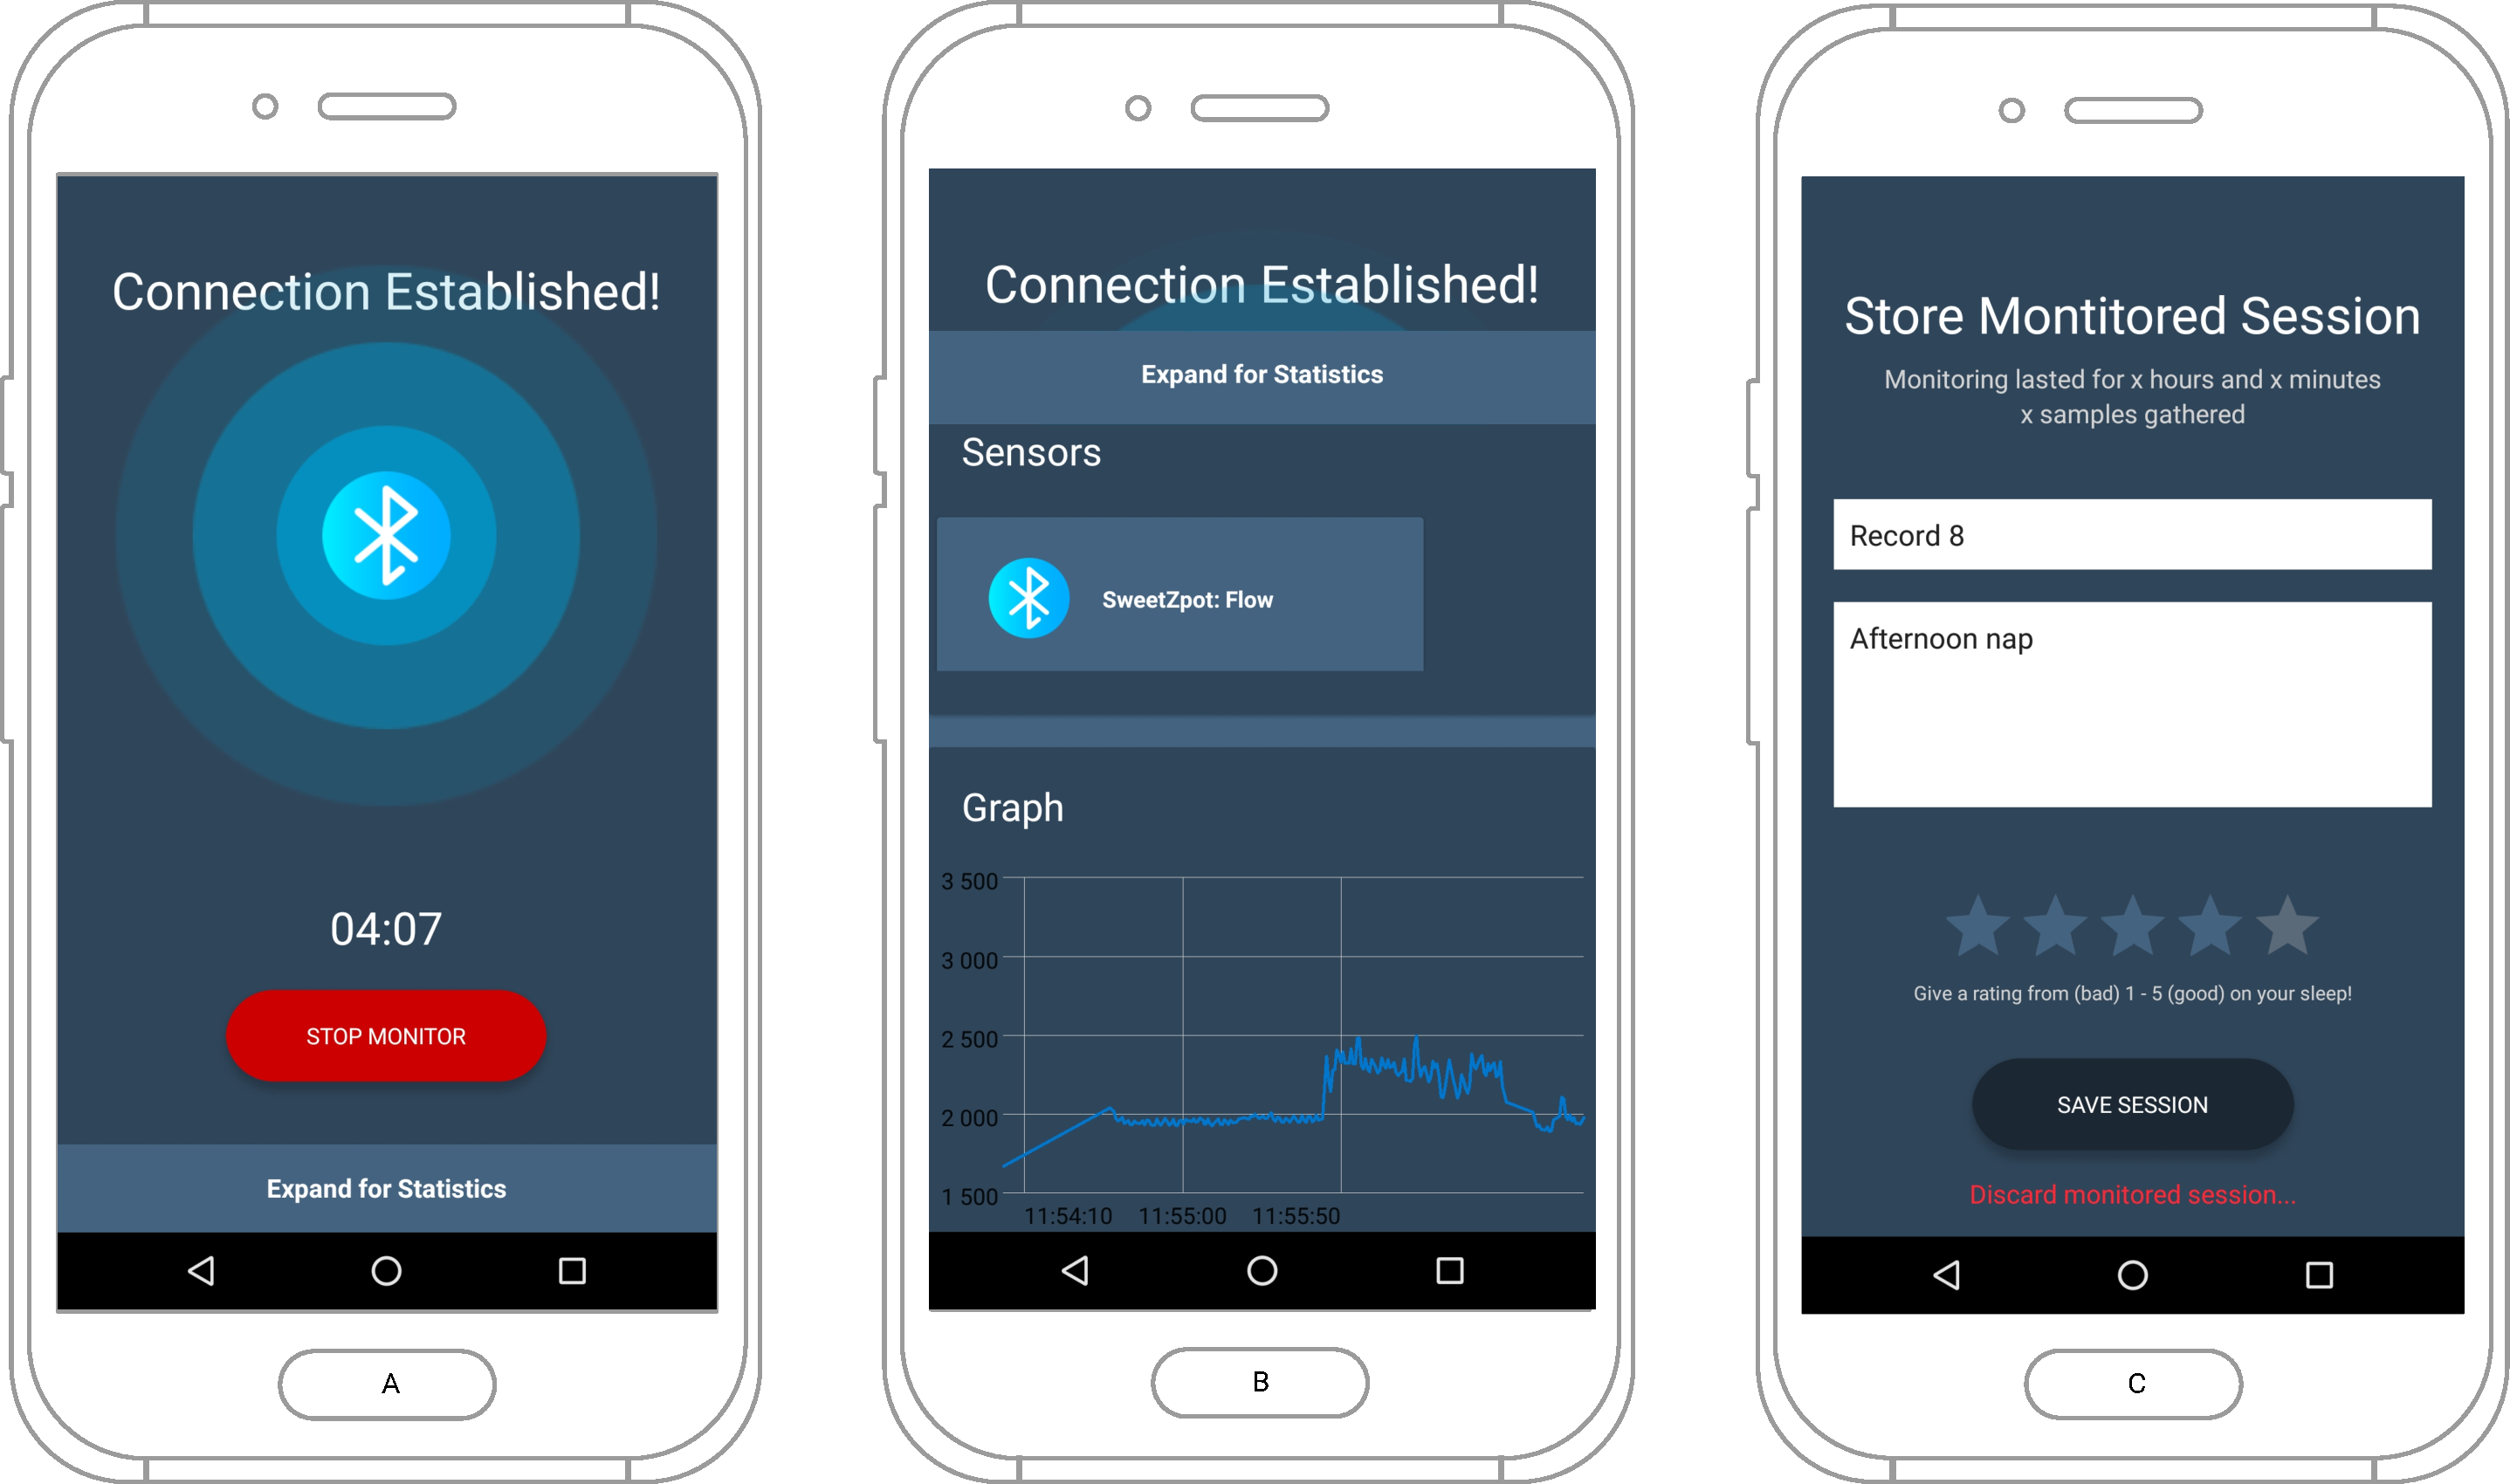
\includegraphics[scale=0.26]{images/Recording_img.pdf}
    \caption{The recording screen displayed to the user: (A) during a recording, (B) statistics interface, and (C) stopping the recording}
    \label{fig:screen_recording}
\end{figure}

\subsubsection{UI: Recording}

Figure \ref{fig:screen_recording} presents the screen for (A) the screen displayed during recording, (B) the interface for statistics, and (C) the screen displayed at the end of the recording. 

\begin{itemize}
    \item[A] The screen displays the elapsed time of recording right below the center of the screen. The button color has a different nuance from the background color to make more distinguishable to the user. On button click, an alert specifying whether the recording should be stopped or not is presented to the user in order to prevent undesired stopping of recording due to misclicks. 
    
    Moreover, the screen has a ripple-effect to indicate the state of the recording to the user. There are two types of ripple-effect colors: a blue ripple-effect indicates for samples acquisition, while a grey ripple-effect indicates that the sensor has disconnected or trying to reconnect. The ripple effect is only active if the screen is turned on in order to preserve battery life. 
    
    As a side note, during disconnects between the sensor and the device, the user provides no extra input to resolve the issue. The attempts to reconnect occurs in the background, and the only state of change is the ripple-effect color. 
    \item[B] The user can expand the interface for viewing statistics with information about the recording. Currently, the interface lists all of the available sensor sources, also a real-time interactable graph of breathing data.
    \item[C] The finalizing screen allows users to specify the title and description of recording, as well as giving a rating between the values of 1--5 (where one is bad, and five is good). Upon saving the recording, the user is transitioned to the \verb|MainActivity|.

\end{itemize}

\subsubsection{UI: Sharing}
\begin{figure}[!h]
    \centering
    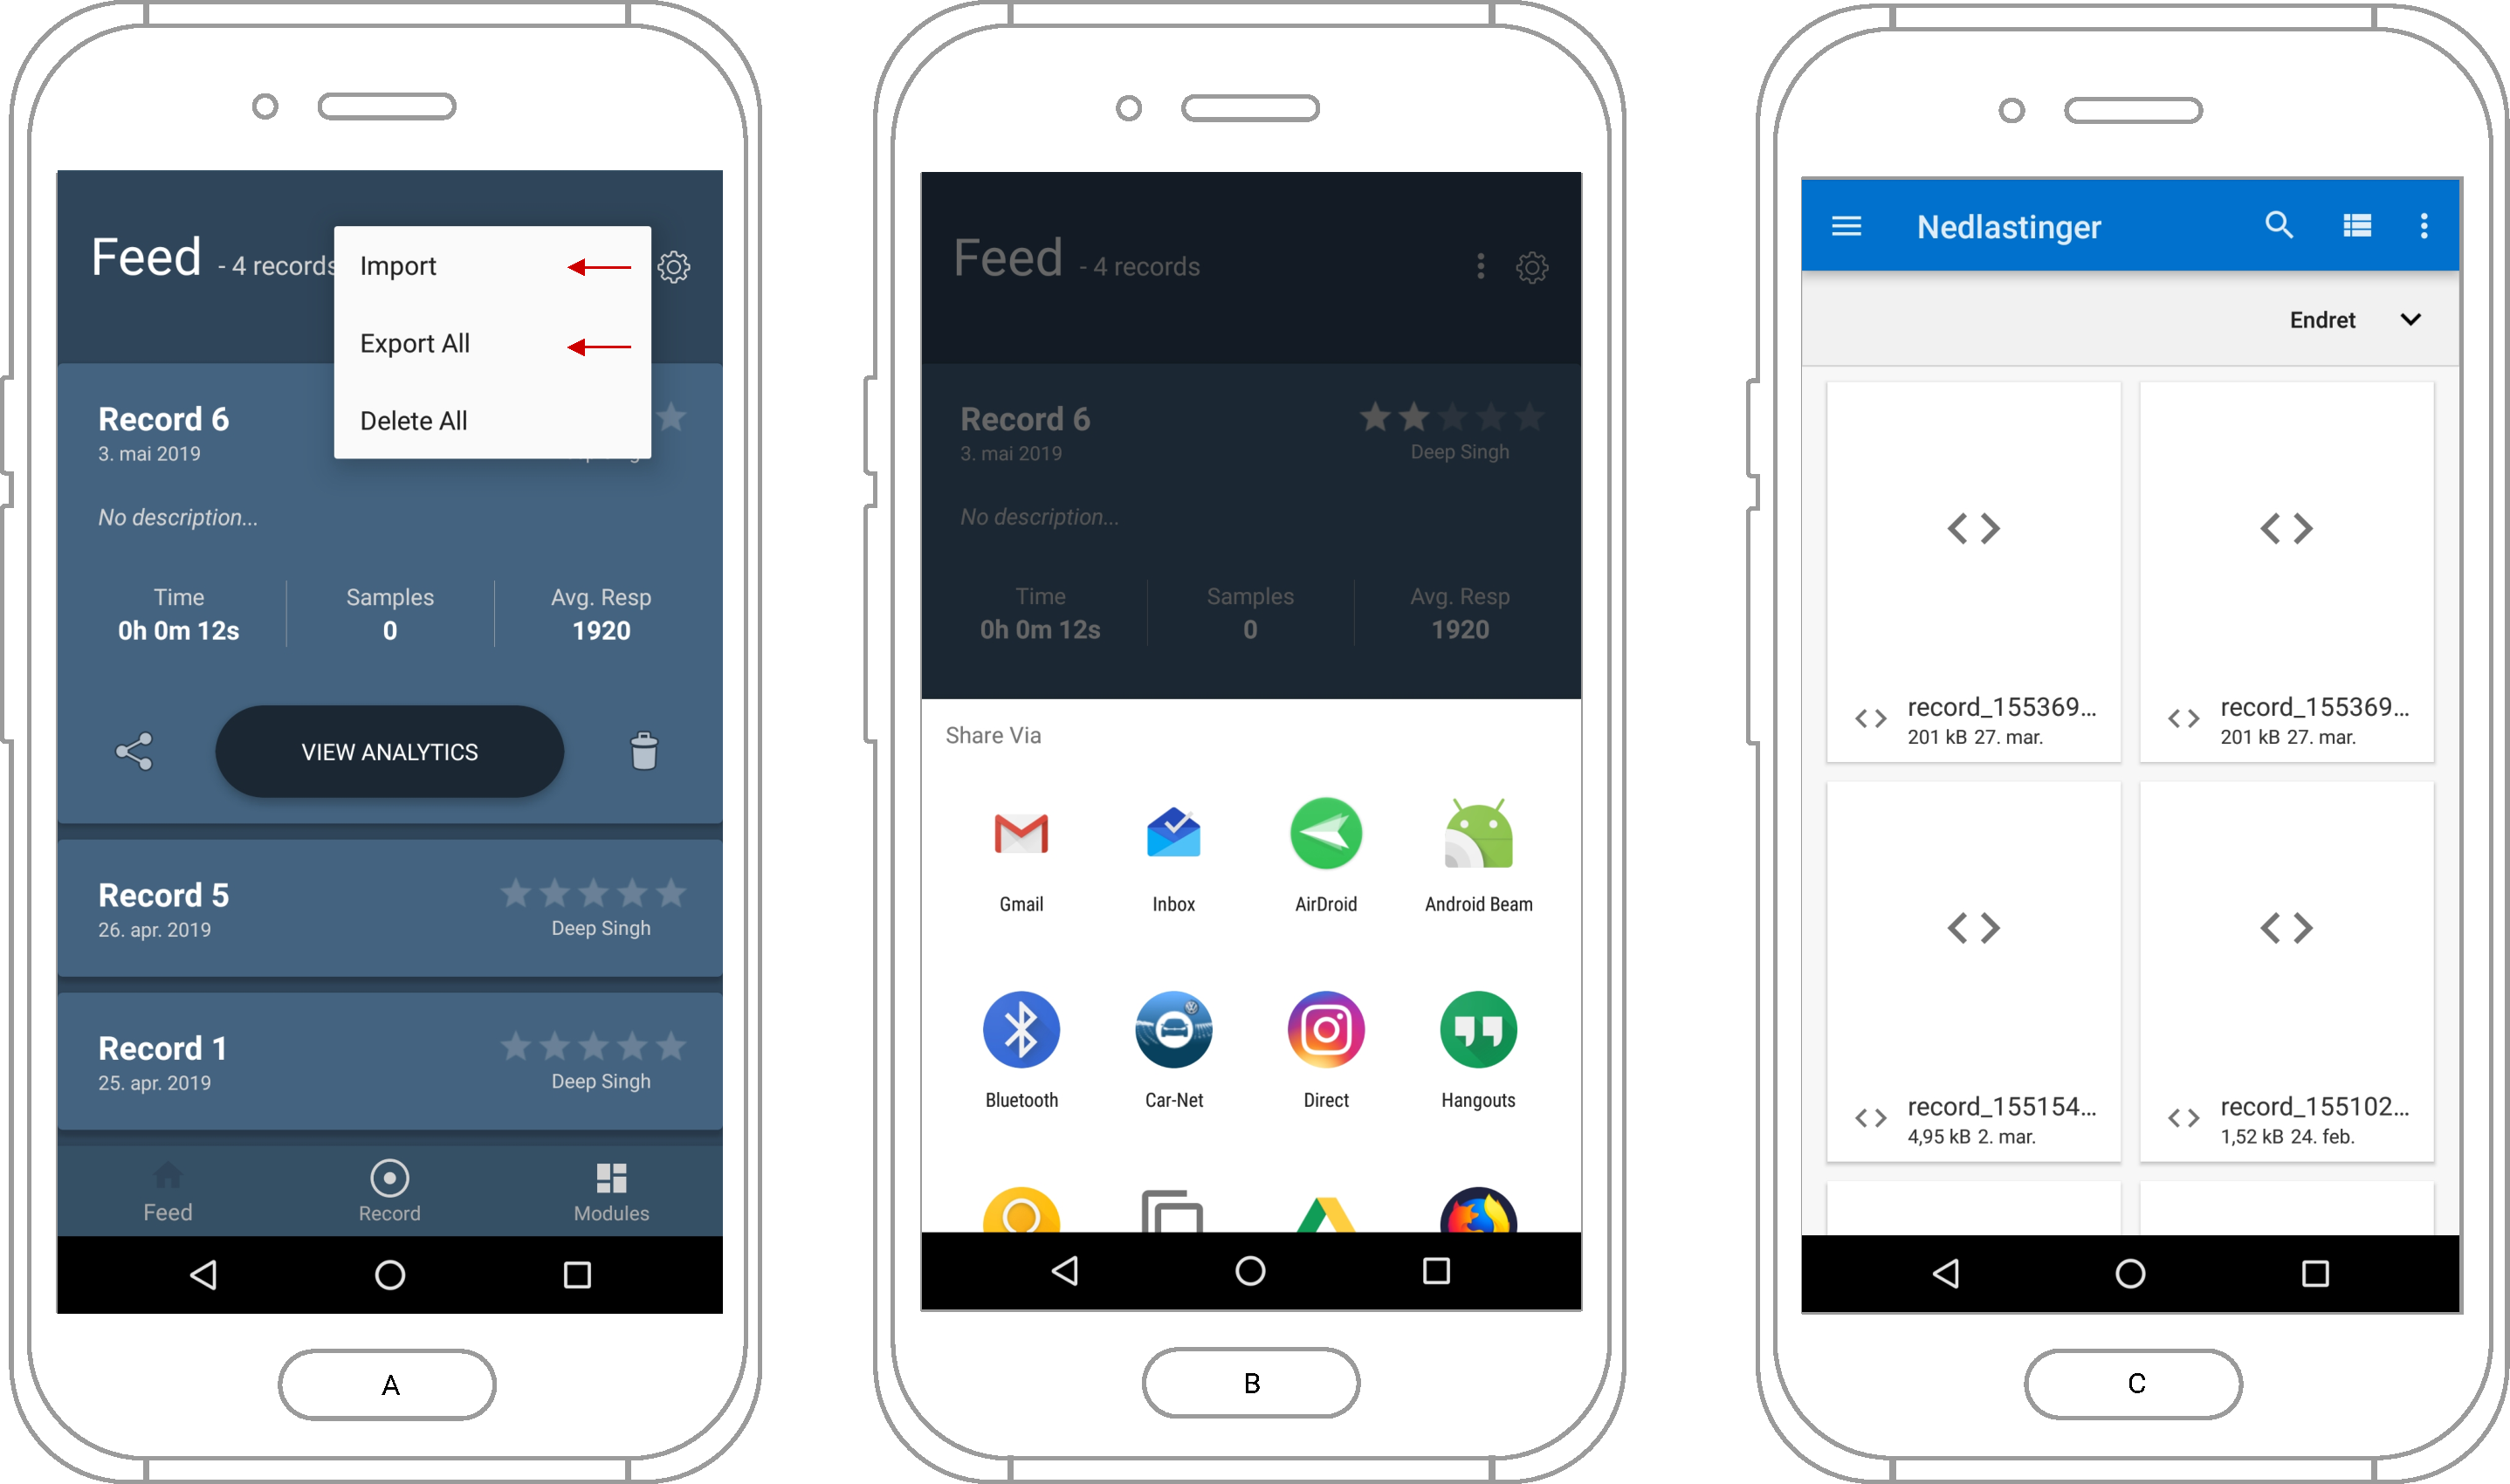
\includegraphics[scale=0.26]{images/Sharing_img.pdf}
    \caption{The sharing screen displayed to the user: (A) option to import or export, (B) the media selection for exporting, and (C) the file selection for importing.}
    \label{fig:screen_sharing}
\end{figure}

Figure \ref{fig:screen_sharing} presents the screen for: (A) option to import or export, (B) the media selection for exporting, and (C) the file selection for importing.

\begin{itemize}
    \item[A] The feed screen is where all of the records are presented to the user as a list. The items in the list are expandable and collapsible to prevent fluttering on the screen, as well as displaying the most important information to the user. The user can press the share icon on a given record, or press on the options menu at the top of the screen to export all or import records.
    \item[B] By pressing export all (or export on a single record), an overlay with an Android provided sharing screen is presented. The interface lists of all applications that provide a method of sharing data, and to us, the e-mail application is the most interesting method to use for sending records. 
    \item[C] By pressing import, an interface that presents all of the downloaded files on the user's device is shown to the user. The user can press on the desired file, and the file will be parsed and added to the user's collection of records.  
\end{itemize}

\subsubsection{UI: Modules}
\begin{figure}[!h]
    \centering
    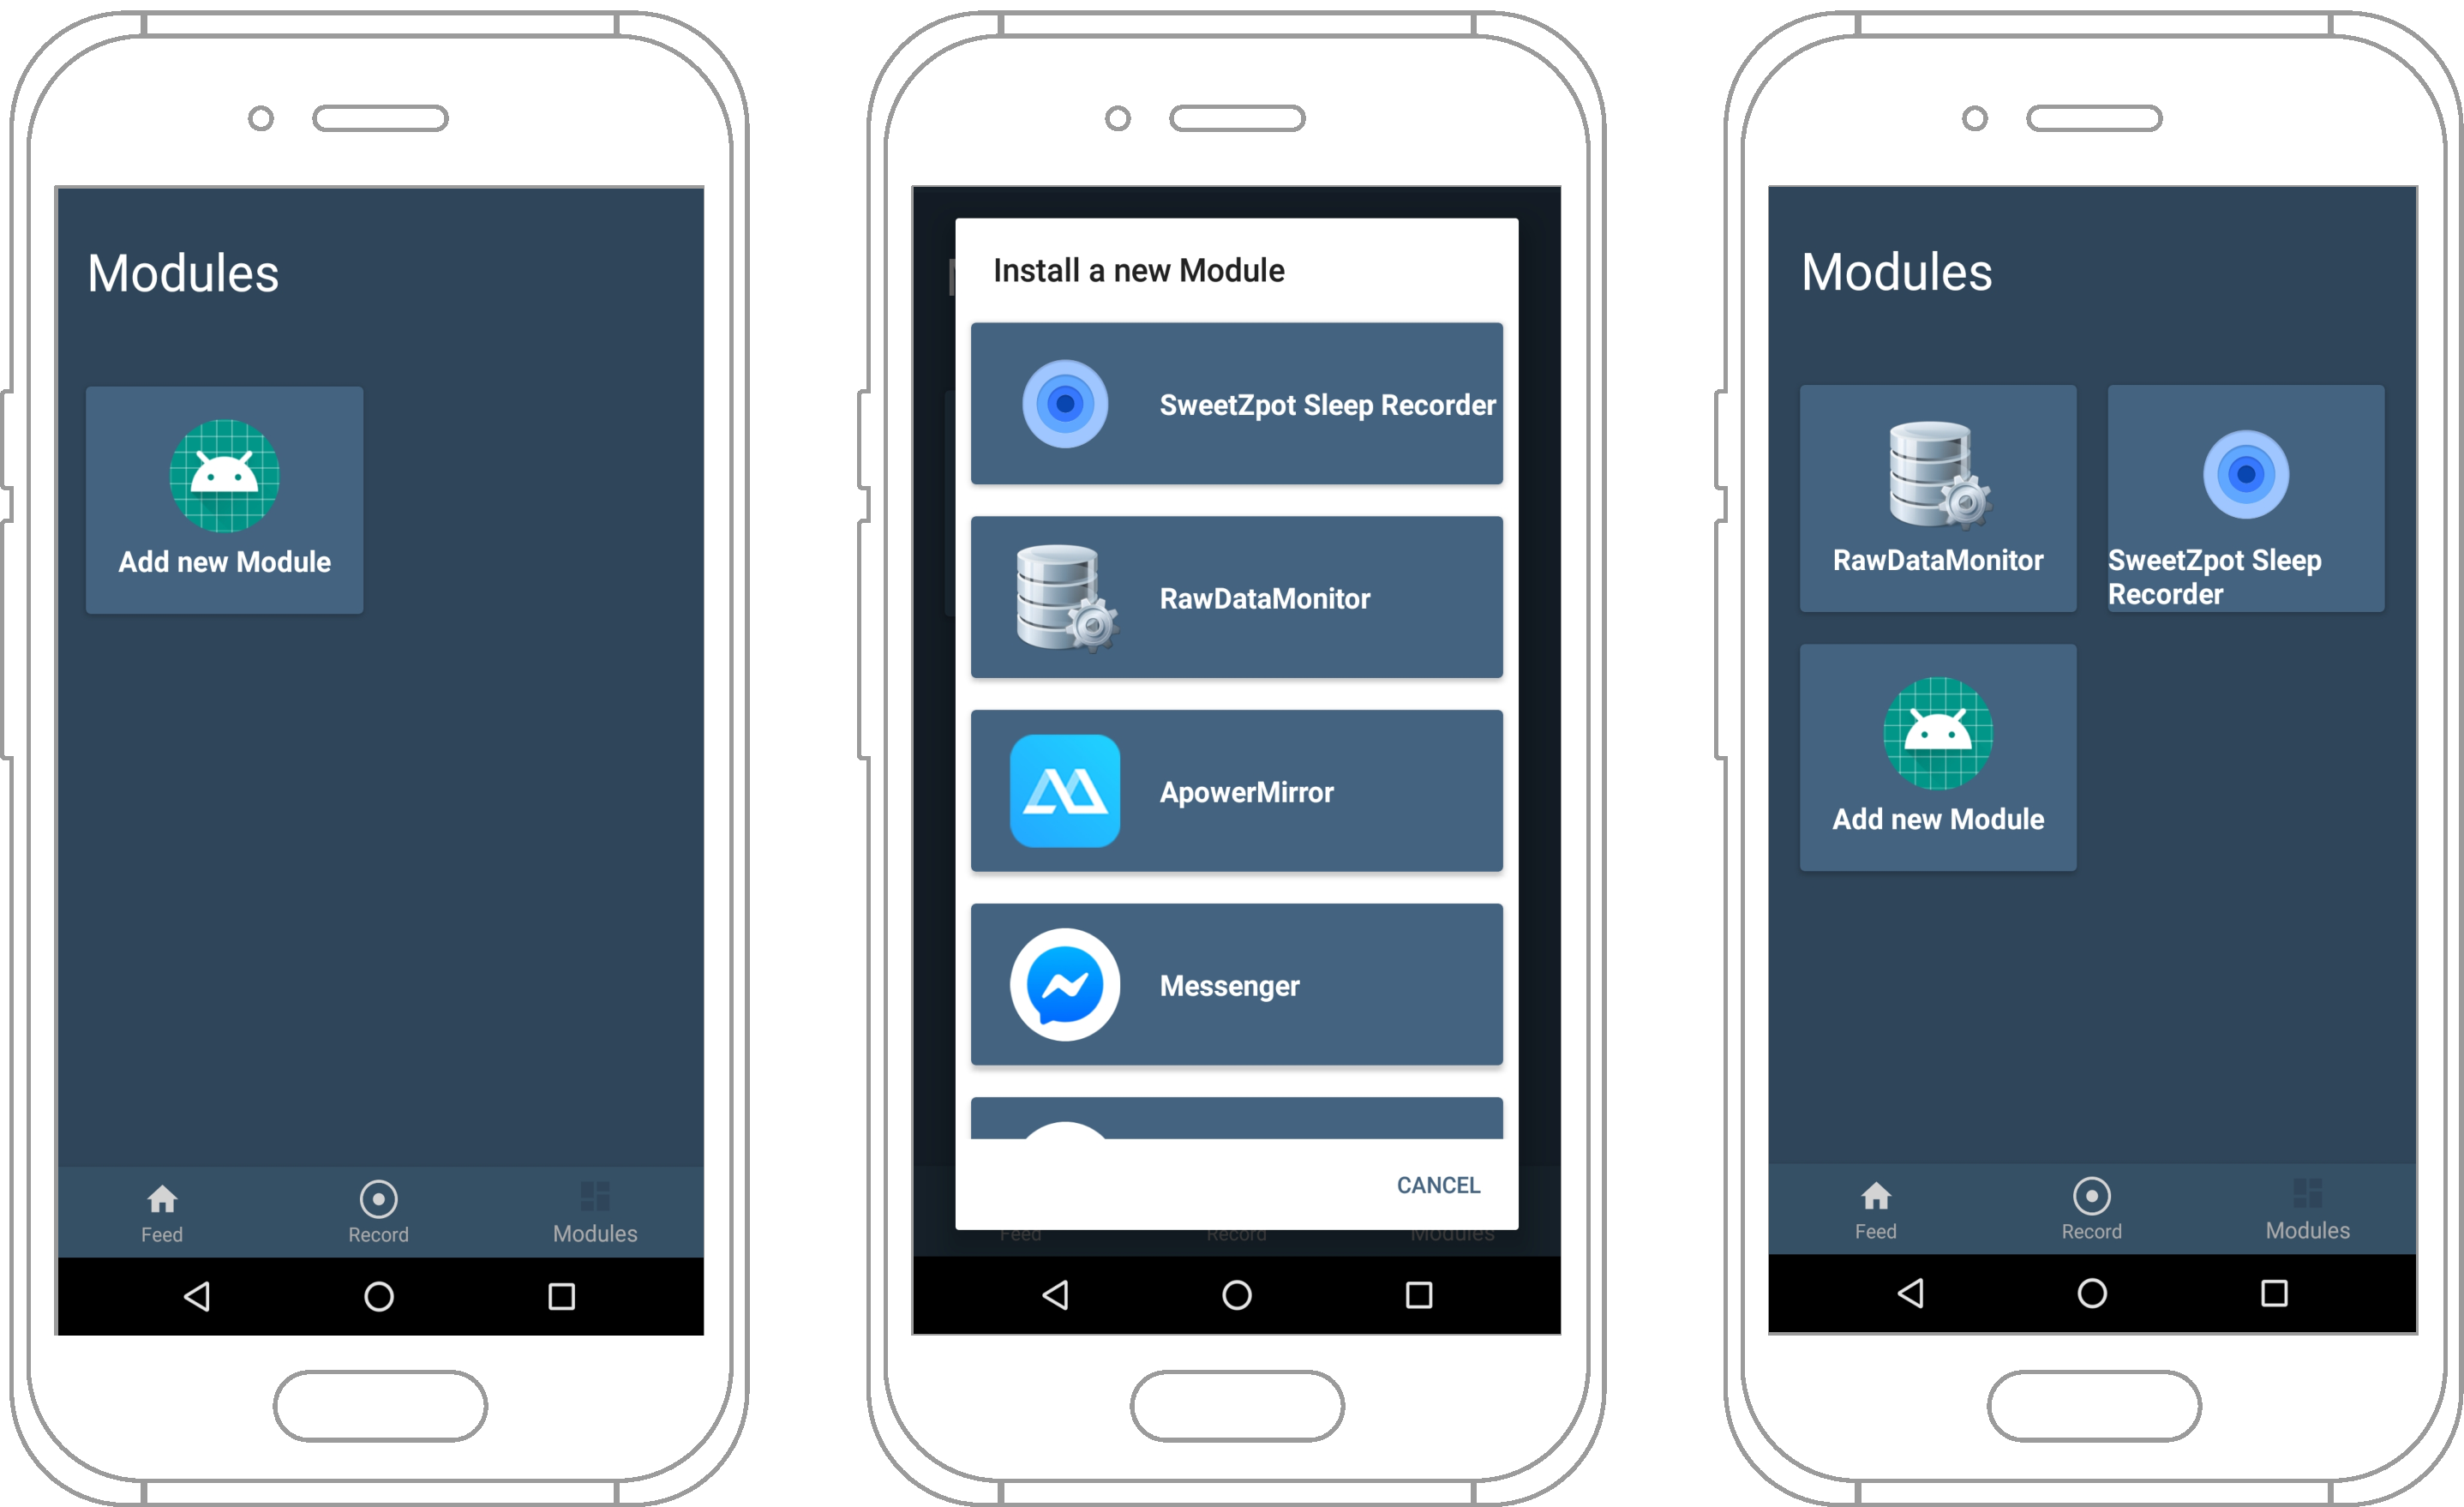
\includegraphics[scale=0.26]{images/Modules_img.pdf}
    \caption{The module screen displayed to the user: (A) module screen without any modules, (B) list of installed applications on the device, and (C) module screen with modules.}
    \label{fig:screen_modules}
\end{figure}

Figure \ref{fig:screen_modules} shows the screen for (A) module screen without any modules, (B) list of installed applications on the device, and (C) module screen with modules. 

\begin{itemize}
    \item[A] The modules screen without any installed modules; however, a button for adding new modules.
    \item[B] The user can press the \textit{add new module} button, in order to be presented with a list of all installed applications. 
    \item[C] Once the user has selected a module-application to be added in Nidra, the list of modules are updated and presented to the user. The modules are hereafter added in Nidra and can be launched by clicking on the module. The module can also be removed by long-pressing (holding down for at least 2 seconds) the module-button.
\end{itemize}

\subsubsection{UI: Analytics}
Figure \ref{fig:screen_analytics} shows the screen for (A) feed screen with a record expanded and (B) the analytics for the record

\begin{itemize}
    \item[A] The user can expand the records to view more information and actions. One of the actions is to view the analytics for the record.
    \item[B] A new screen with an interactable graph, that is populated with the samples associated with the selected record, is presented to the users. The graph shows the respiration (breathing) value (Y-axis) on given time (X-axis) of sampling. Also, information on the number of samples and elapsed time of recording. 
\end{itemize}

\begin{figure}[!h]
    \centering
    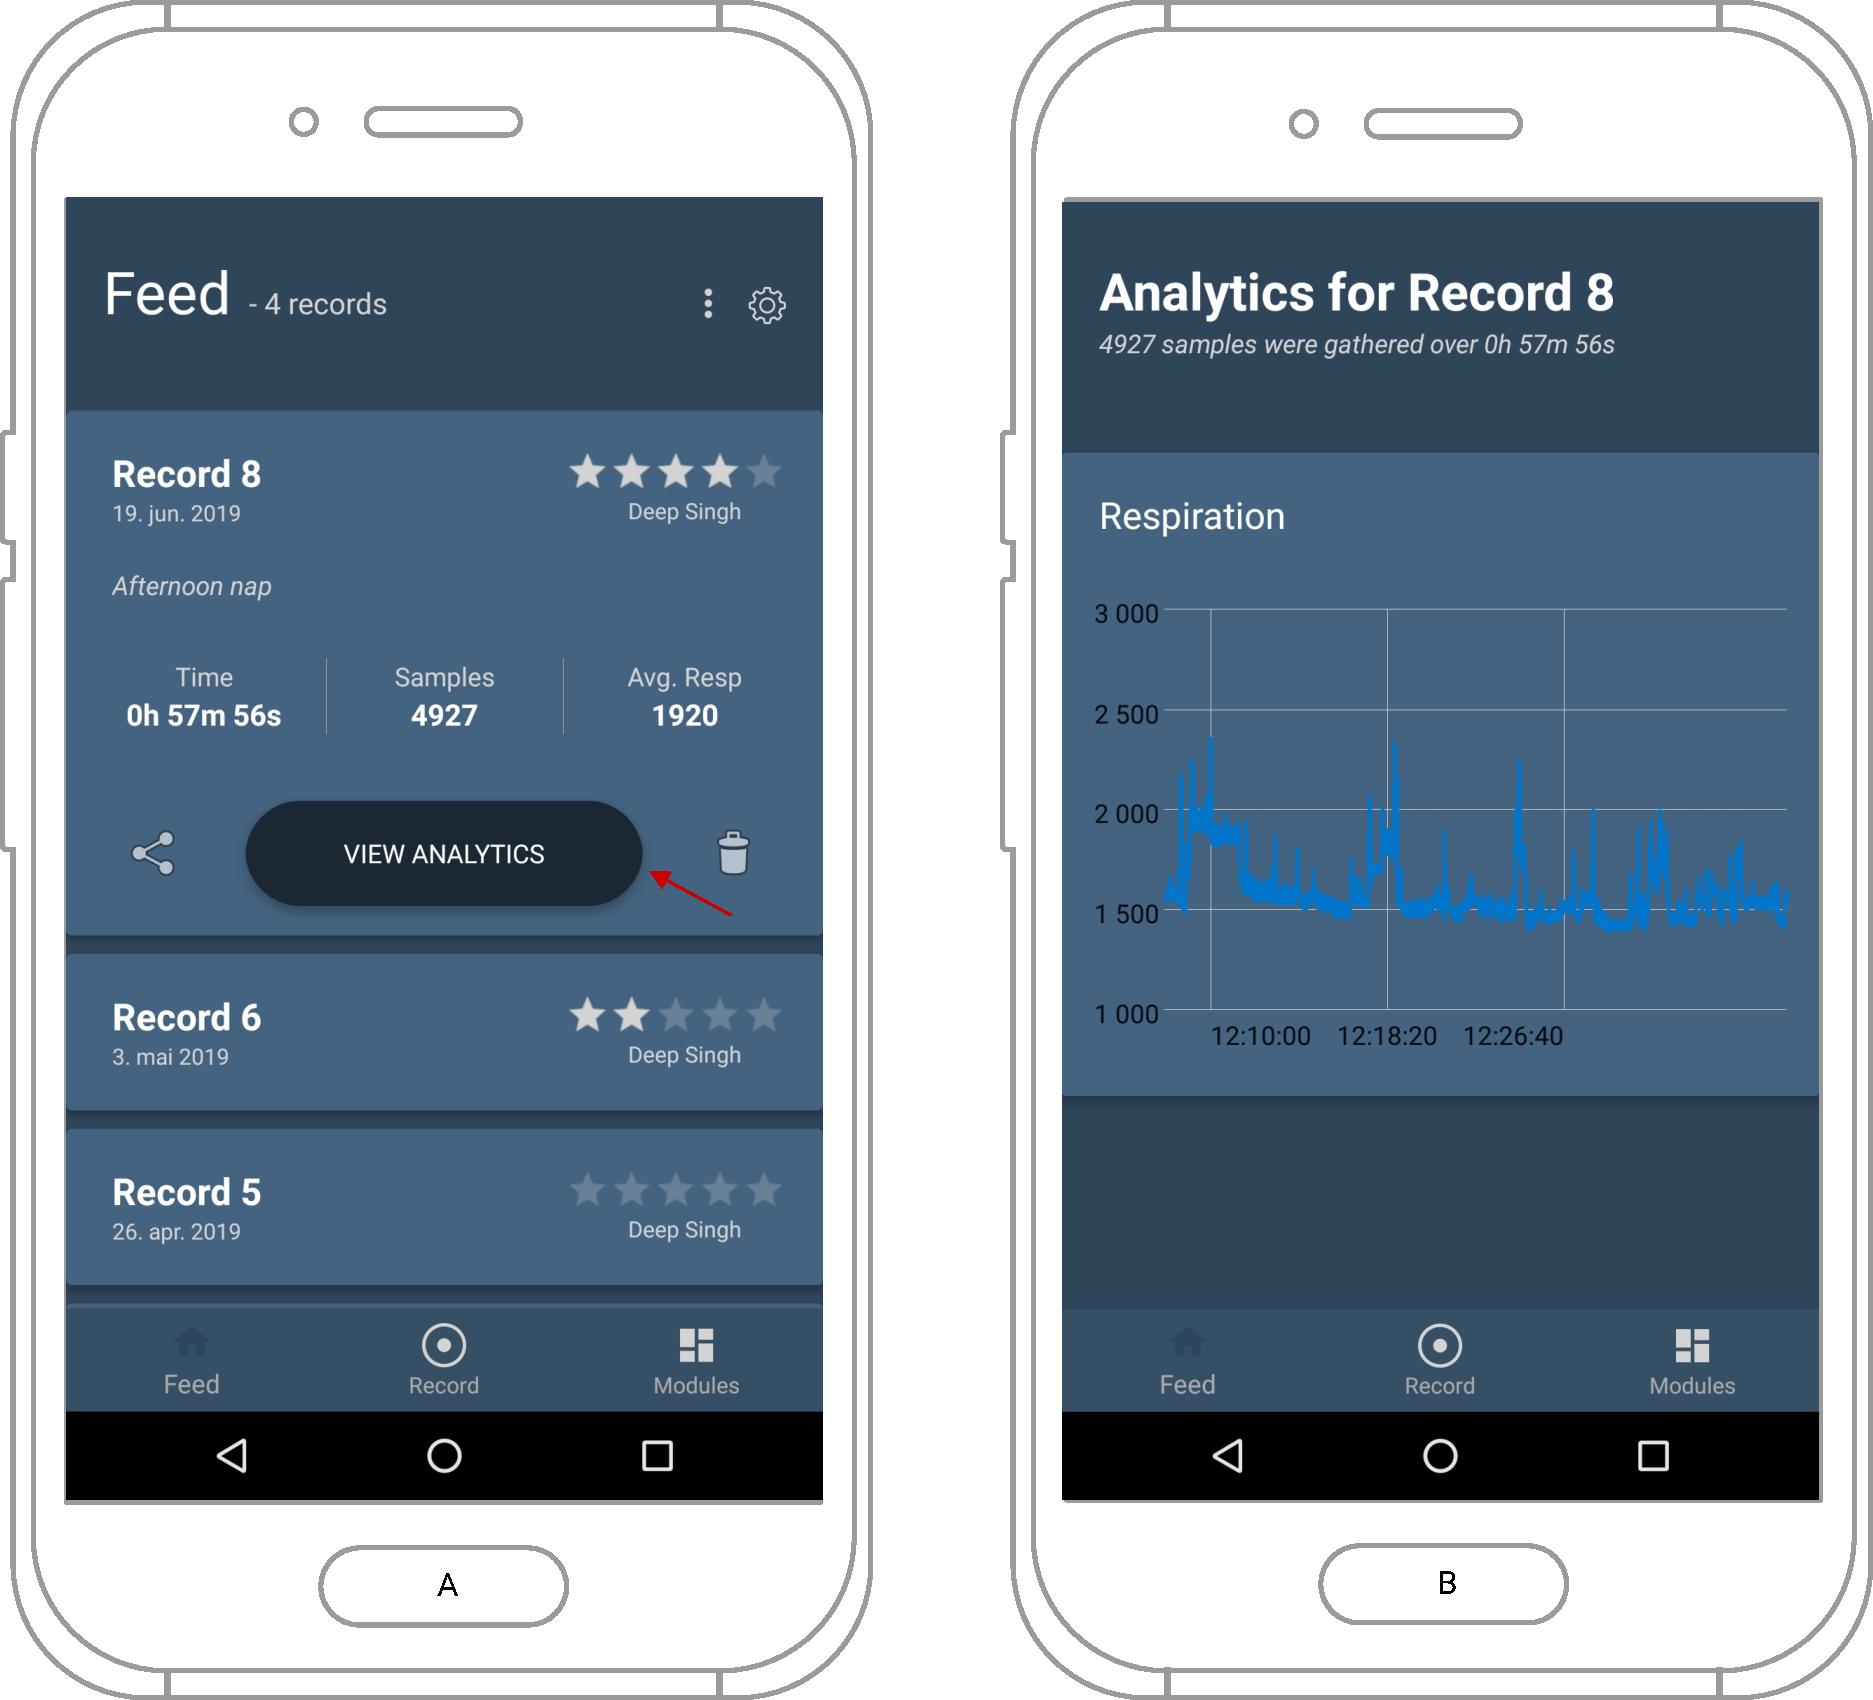
\includegraphics[scale=0.26]{images/Analytics_img.pdf}
    \caption{The analytics screen displayed to the user: (A) the feed screen; (B) the analytics screen}
    \label{fig:screen_analytics}
\end{figure}
